\documentclass[10pt, a4paper]{article}
\usepackage[paper=a4paper, left=1.5cm, right=1.5cm, bottom=2.5cm, top=3.5cm]{geometry}
\usepackage{fancyhdr}
\usepackage[spanish,activeacute]{babel}
\pagestyle{fancy}
\frenchspacing
\usepackage[dvips]{graphicx}
%~ \usepackage[dvips]{geometry}
\usepackage[usenames]{color}
\usepackage{colortbl}
\usepackage{amssymb}
\usepackage{caratula}
\usepackage{hyperref}
\usepackage[utf8]{inputenc}
\usepackage{array}
\usepackage{float}

\hypersetup{%
 pdfauthor={Hernandez, Laurito, Capello},
 pdfsubject={TP2 redes}
}

% Acomodo fancyhdr <- El encabezado de pagina
\pagestyle{fancy}
\thispagestyle{fancy}
\addtolength{\headheight}{1pt}
\lhead{Teoría de las comunicaciones - TP2}
\rhead{Primer Cuatrimestre 2013}
\cfoot{\thepage}
\renewcommand{\footrulewidth}{0.4pt}

%~ \lhead{\textbf{Teoría de las comunicaciones - TP2}}
%~ \rhead{Capello - Hernandez - Laurito}
%~ \lfoot{Taller de capa de red}
%~ \rfoot{\thepage}
%~ \cfoot{ }
%~ \renewcommand{\headrulewidth}{0.6pt}
%~ \renewcommand{\footrulewidth}{0.4pt}
%~ \addtolength{\textwidth}{2cm}
%~ \addtolength{\hoffset}{-0.8cm}
%~ \fancyheadoffset{1cm}
%~ \fancyfootoffset{1cm}

\begin{document}

% Caratula
\materia{Teor'ia de las Comunicaciones}
\submateria{Primer Cuatrimestre de 2013}
\titulo{Tp2: capa de red}
%\subtitulo{}
\grupo{Grupo:}
\integrante{Andr'es Laurito}{27/11}{andy.laurito@hotmail.com}
\integrante{Mat\'ias Capello}{006/02}{matiascapello@gmail.com}
\integrante{Santiago Hern'andez}{48/11}{santi-hernandez@hotmail.com}

\thispagestyle{empty}
\begin{titlepage}
\maketitle
\thispagestyle{empty}
\end{titlepage} 
\newpage

% Indice, indice figuras, comienzo
\thispagestyle{fancy}
\tableofcontents
\newpage
\listoffigures
\newpage

% Secciones
\section*{\centering Abstract}

{\em
En este taller experimentamos con herramientas y t'ecnicas frecuentes a nivel de red. En la primera parte desarrollamos nuestras propias implementaciones de ping y traceroute.
En la segunda parte utilizamos dichas implementaciones para encontrar enlaces transatl'anticos. Se calcul'o la distancia lineal de dichos enlaces
y se analiz'o el RTT real en distintos momentos del d'ia. Se encontraron dificultades para encontrar los enlaces solicitados, las que se atribuyen a diferentes posibles razones, 
como la existencia de t'uneles que ocultan los verdaderos enlaces, restricciones de ruteo de los ISPs utilizados, falta de precisi'on de los
servicios de geolocalizaci'on. Con respecto a la variaci'on del RTT a lo largo del d'ia, si bien se observa una cierta estabilidad en su mayor'ia, 
se ven algunos picos de mayor RTT, lo que estar'ia relacionado con horarios pico de uso del enlace.
}


\section{Introducción}

En este taller nos proponemos experimentar con herramientas y técnicas frecuentes a nivel de red. Más particularmente nos centraremos en dos muy conocidas y utilizadas: \texttt{ping} y \texttt{traceroute}. El objetivo es entender los protocolos involucrados. Para ello, desarrollaremos nuestras propias implementaciones de las herramientas de manera de afianzar los conocimientos. Todo lo anterior se realizará en un marco analítico que nos permitirá razonar sobre lo hecho y comprender mejor qué pasa detrás de bambalinas.

\subsection{ICMP}

El Protocolo de Mensajes de Control de Internet o ICMP es el sub protocolo de control y notificación de errores del Protocolo de Internet (IP). Como tal, se usa para enviar mensajes de error, indicando por ejemplo que un servicio determinado no está disponible o que un router o host no puede ser localizado.

ICMP difiere del propósito de TCP y UDP ya que generalmente no se utiliza directamente por las aplicaciones de usuario en la red. La única excepción es la herramienta \texttt{ping} y \texttt{traceroute}, que envían mensajes de petición Echo ICMP (y recibe mensajes de respuesta Echo) para determinar si un host está disponible, el tiempo que le toma a los paquetes en ir y regresar a ese host y cantidad de hosts por los que pasa.

\vspace*{5 mm}

Los mensajes ICMP son comúnmente generados en respuesta a errores en los datagramas de IP o para diagnóstico y ruteo. IP encapsula el mensaje ICMP apropiado con una nueva cabecera IP (para obtener los mensajes de respuesta desde el host original que envía), y transmite el datagrama resultante de manera habitual.

Por ejemplo, cada router que reenvía un datagrama IP tiene que disminuir el campo de tiempo de vida (TTL) de la cabecera IP en una unidad; si el TTL llega a 0, un mensaje ICMP ''Tiempo de Vida se ha excedido en transmitirse'' es enviado a la fuente del datagrama. Cada mensaje ICMP es encapsulado directamente en un solo datagrama IP, y por tanto no garantiza la entrega del ICMP. Aunque los mensajes ICMP son contenidos dentro de datagramas estándar IP, los mensajes ICMP se procesan como un caso especial del procesamiento normal de IP, algo así como el procesamiento de un sub-protocolo de IP. En muchos casos es necesario inspeccionar el contenido del mensaje ICMP y entregar el mensaje apropiado de error a la aplicación que generó el paquete IP original, aquel que solicitó el envío del mensaje ICMP.

\vspace*{5 mm}

La utilidad del protocolo ICMP es controlar si un paquete no puede alcanzar su destino, si su vida ha expirado, etc. Es decir, se usa para manejar mensajes de error y de control necesarios para los sistemas de la red, informando con ellos a la fuente original para que evite o corrija el problema detectado.

Muchas de las utilidades de red comunes están basadas en los mensajes ICMP. El comando \texttt{traceroute} está implementado transmitiendo datagramas UDP con campos especiales TTL IP en la cabecera, y buscando los mensajes de ''Tiempo de Vida en tránsito'' y ''Destino inalcanzable'' generados como respuesta. La herramienta \texttt{ping} está implementada utilizando los mensajes ''Echo request'' y ''Echo reply'' de ICMP.

\subsection{Ping}

Como programa, \texttt{ping} es una utilidad de diagnóstico en redes de computadoras que comprueba el estado de la comunicación del host local con uno o varios equipos remotos de una red TCP/IP por medio del envío de paquetes ICMP de solicitud y de respuesta. Mediante esta utilidad puede diagnosticarse el estado, velocidad y calidad de una red determinada.

\vspace*{5 mm}

Ejecutando \texttt{ping} de solicitud, el Host local envía un mensaje ICMP, incrustado en un paquete IP. El mensaje ICMP de solicitud incluye, además del tipo de mensaje y el código del mismo, un número identificador y una secuencia de números, de 32 bits, que deberán coincidir con el mensaje ICMP de respuesta; además de un espacio opcional para datos. Muchas veces se utiliza para medir la latencia o tiempo que tardan en comunicarse dos puntos remotos.

\subsection{Traceroute}

\texttt{traceroute} es una consola de diagnóstico que permite seguir la pista de los paquetes que vienen desde un host (punto de red). Se obtiene además una estadística del RTT o latencia de red de esos paquetes, lo que viene a ser una estimación de la distancia a la que están los extremos de la comunicación. 

\vspace*{5 mm}

Entre los datos que se obtienen están: el número de salto, el nombre y la dirección IP del nodo por el que pasa y el tiempo de respuesta para los paquetes enviados (un asterisco indica que no se obtuvo respuesta).

\texttt{traceroute} utiliza el campo Time To Live (TTL) de la cabecera IP. Este campo sirve para que un paquete no permanezca en la red de forma indefinida (por ejemplo, debido a la existencia en la red de un bucle cerrado en la ruta). El campo TTL es un número entero que es decrementado por cada nodo por el que pasa el paquete. De esta forma, cuando el campo TTL llega al valor 0 ya no se reenviará más, sino que el nodo que lo esté manejando en ese momento lo descartará. Lo que hace \texttt{traceroute} es mandar paquetes a la red de forma que el primer paquete lleve un valor TTL=1, el segundo un TTL=2, etc. De esta forma, el primer paquete será eliminado por el primer nodo al que llegue (ya que éste nodo decrementará el valor TTL, llegando a cero). Cuando un nodo elimina un paquete, envía al emisor un mensaje de control especial indicando una incidencia. \texttt{traceroute} usa esta respuesta para averiguar la dirección IP del nodo que desechó el paquete, que será el primer nodo de la red. La segunda vez que se manda un paquete, el TTL vale 2, por lo que pasará el primer nodo y llegará al segundo, donde será descartado, devolviendo de nuevo un mensaje de control. Esto se hace de forma sucesiva hasta que el paquete llega a su destino.

\section{Desarrollo}

\subsection{Implementación ping}

como esta en las diapositivas

\subsection{Implementación traceroute}

como esta en las diapositivas

\subsubsection{Geolocalización direcciones IP}

Para geolocalizar la dirección IP de las respuestas obtenidas al hacer el traceroute utilizamos el servicio gratuito provisto por \textbf{dazzlepod.com/ip} una vez obtenida la respuesta, quien nos devuelve entre otros datos, las coordenadas terrestres aproximadas de la posición de la ip en un json.

\subsubsection{Calculo de la distancia entre coordenadas}

Una vez obtenidas las coordenadas terrestres de los hops del traceroute utilizamos la \textbf{fórmula del haversine} para calcular la distancia en kilómetros entre un hop y el anterior.	\\
Fórmula de Haversine $ = 2 * r * arcsin \left (\sqrt{sin^{2} \left (\frac{\phi_{1}-\phi_{2}}{2}\right ) + cos(\phi_{1}) * cos(\phi_{2}) * sin^{2} \left (\frac{\lambda_{1}-\lambda_{2}}{2}\right )}\right )$	\\
Donde $r$ es el radio medio de la tierra en kilómetros (en nuestra implementación utilizamos 6371Km), $\phi_{1}$ y $\phi_{2}$ son la latitud de la coordenada 1 y 2, respectivamente, y $\lambda_{1}$ y $\lambda{2}$ son la longitud de la coordenada 1 y 2.

\subsubsection{Calculo del RTT real y teórico}

Para calcular el RTT mínimo suponiendo que los enlaces son de fibra óptico, siendo su tiempo de propagación de $2*10^{5}Km/s$, tomamos la distancia en kilómetros entre los nodos calculadas anteriormente y la dividimos por el tiempo de propagación.	\\
\indent Por otro lado para calcular el RTT real aproximado iniciamos un contador antes de enviar el paquete y lo detenemos al obtener su respuesta correspondiente.

\subsubsection{Gráfico mapa traceroute}

Una vez terminado el traceroute utilizamos la api de \textbf{google static maps} para obtener graficamente en un mapamundi el recorrido realizado para alcanzar el destino. El servicio nos devuelve una imagen en formato png, la cual guardamos, luego de hacer un request a la dirección base de google static maps añadiendole los pins y caminos a agregar.	\\
\indent	Para hacer el pedido utilizamos la dirección base \\http://maps.googleapis.com/maps/api/staticmap?zoom=1\&size=600x400\&scale=2\&sensor=false\&maptype=roadmap	\\
 a la cual le agregamos para cada ip que contesto un pin: \&markers=label:\textbf{label}$|$\textbf{latidud},\textbf{longitud}, y finalmente trazamos los caminos entre las ips que contestaron una después de la otra, también agregando a la dirección \\ \&path=color:0xff0000$|$weight:2$|$ seguido de las coordenadas de cada ip separadas por un pipe ($|$).	\\
\indent Una descripción detallada del uso de google static maps se puede encontrar en: \\ https://developers.google.com/maps/documentation/staticmaps/

\section{Resultados}

\subsection{Enlaces transatlánticos}

%~ \begin{figure}[!hbp]
\begin{figure}[H]
\begin{center}
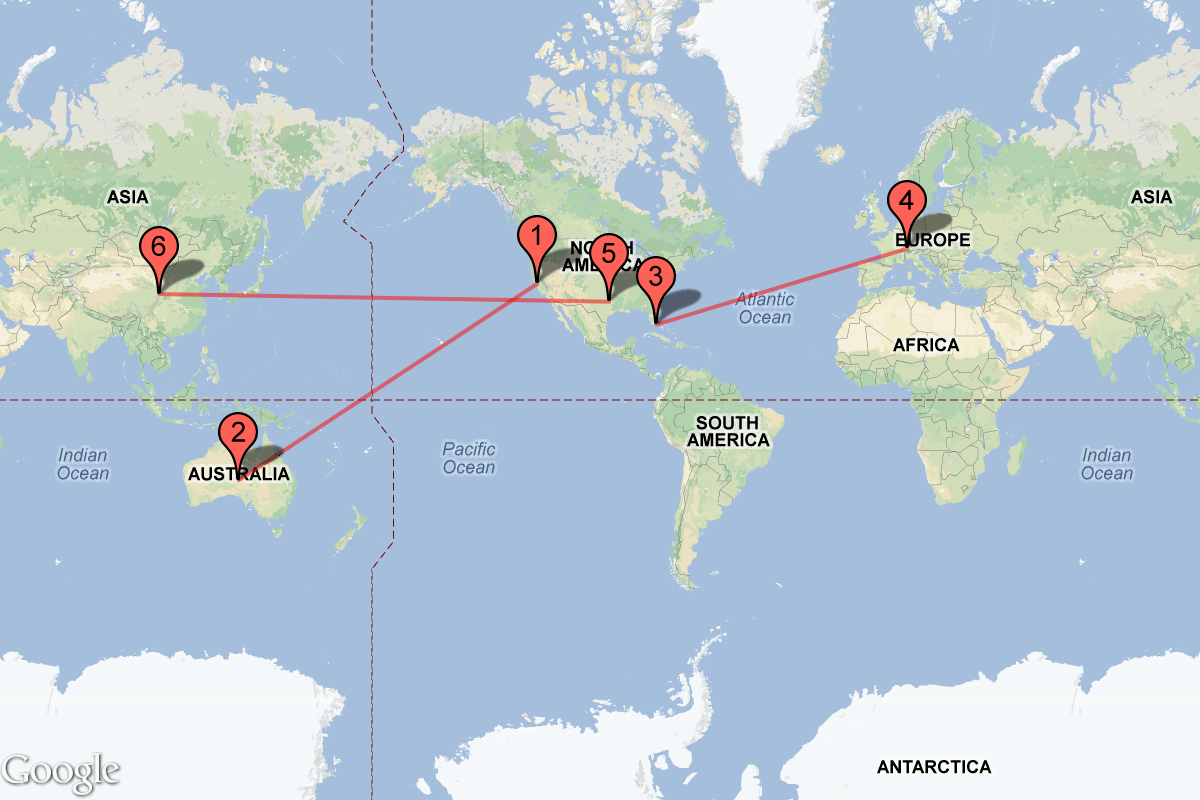
\includegraphics[width=17cm]{enlaces.png}
\end{center}
\caption{Enlaces transatlánticos} \label{figura1}
\end{figure}

\noindent \begin{center} \begin{tabular}{| c | c | c | c | c |} \hline 
Pin 	 & 	 Dirección IP 	 & 	 Coordenadas 	 & 	 Distancia total recorrida hasta él en Km 	 & 	 RTT mínimo en ms \\ \hline 
1 	 & 	 89.221.35.141 	 & 	 (37.9283,-122.0566) 	 & 	 11179.8250554 	 & 	 55.9 \\ \hline 
2 	 & 	 202.158.194.173 	 & 	 (-27.0,133.0) 	 & 	 24234.7289268 	 & 	 121.17 \\ \hline 
3 	 & 	 195.22.199.109 	 & 	 (25.7743,-80.1937) 	 & 	 7887.31191972 	 & 	 39.44 \\ \hline 
4 	 & 	 195.2.6.169 	 & 	 (47.0,8.0) 	 & 	 15702.4500297 	 & 	 78.51 \\ \hline 
5 	 & 	 89.221.40.131 	 & 	 (32.7831,-96.8067) 	 & 	 9285.34331745 	 & 	 46.43 \\ \hline 
6 	 & 	 219.158.33.189 	 & 	 (35.0,105.0) 	 & 	 21427.6048813 	 & 	 107.14 \\ \hline 
\end{tabular} \end{center}

\noindent \begin{center} \begin{tabular}{| c | c | c | c | c |} \hline 
Enlace 	 &	Distancia en Km 	& 	RTT mínimo en ms	\\ \hline 
1 - 2	 &	13054.90 	 		& 	65.27				\\ \hline 
3 - 4 	 & 	7815.13	 			& 	39.07				\\ \hline 
5 - 6 	 & 	12142.26 			&	60.71				\\ \hline 
\end{tabular} \end{center}

\subsection{Variación del RTT a lo largo del día}

Hacer pings a los 6 ips de los enlaces a lo largo del dia

\subsection{Casos curiosos}

%~ \begin{figure}[!hbp]
\begin{figure}[H]
\begin{center}
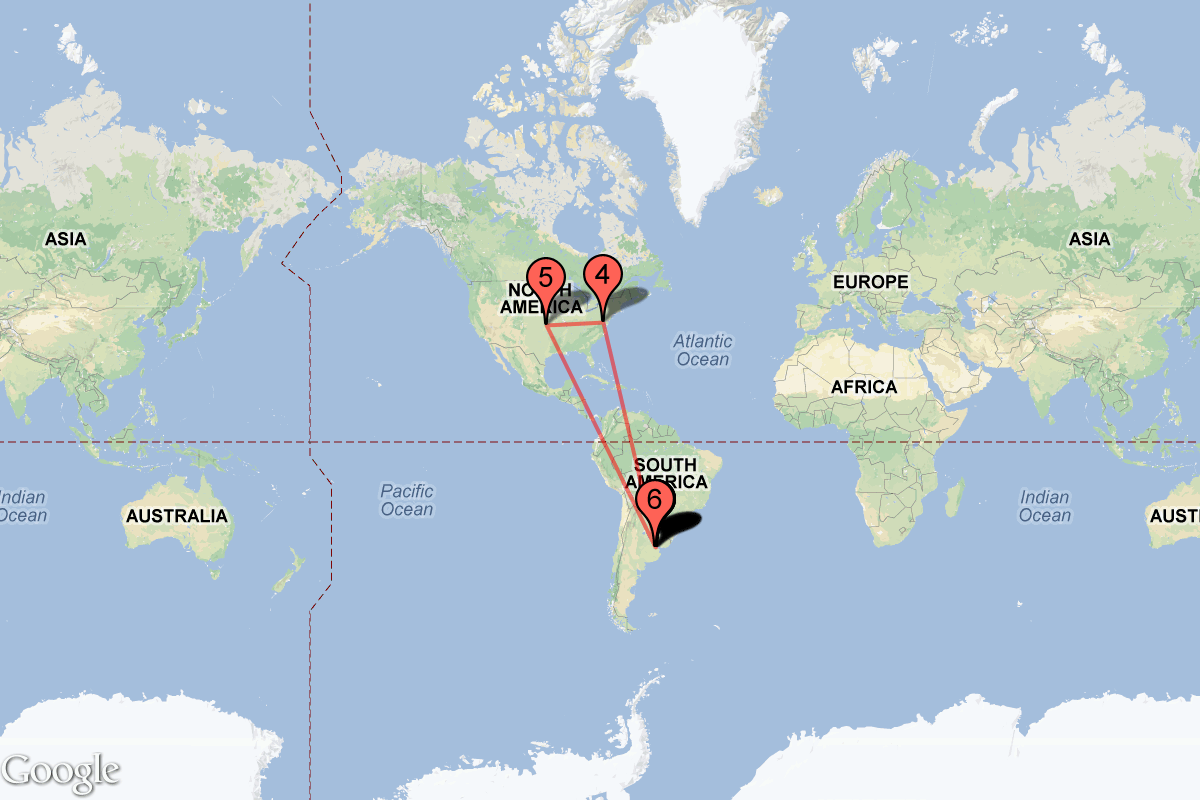
\includegraphics[width=17cm]{perfil.png}
\end{center}
\caption{Traceroute a perfil.com.ar} \label{figura1}
\end{figure}



\section{Análisis de resultados}

Si bien en submarinecablemap.com se ve una gran cantidad de enlaces que cruzan el atl'antico, notamos que s'olo un par son los utilizados para llegar del otro lado del oc'eano. Suponemos que 'esto puede estar relacionado con los ISPs utilizados (telecentro, fibertel). Incluso en pruebas que trataron de forzar el uso de los enlaces que van a Africa desde Brasil, el resultado inclu'ia un enlace USA - Londres. Esto tambi'en puede indicar que estos enlaces sean de mayor velocidad que los anteriores, por lo que son los elegidos para llegar a destino.

Como se puede ver en la figura 2 \ref{figura2}, a lo largo del día en todos los enlaces el RTT hacia el extremo del enlace en los Estados Unidos es menor al del RTT hacia el extremo del enlace perteneciente a Europa, lo que se corresponde con que ambos pertenezcan al mismo enlace.	\\
A su vez podemos observar que la diferencia entre los RTTs es considerablemente superior al RTT mínimo esperado, por lo que podemos suponer que gran parte de la diferencia entre los RTTs de los extremos del enlace y el RTT mínimo esperado, sea el tiempo de ser despachado de un extremo al otro, es decir:	\\
\begin{displaymath}
   RTT_{Europa} - RTT_{USA} - RTT_{USA/Europa minimo} = T_{Queue Usa}
\end{displaymath}

\section{Conclusiones}



\end{document}

